% Compilation : pdflatex B5.tex (deux fois).
% Document autonome : texte, formules et figures TikZ modifiables.
% Les repères « Manuscrit » renvoient aux pages du manuscrit.
\documentclass[11pt,a4paper]{article}
\usepackage[utf8]{inputenc}
\usepackage[T1]{fontenc}
\usepackage[provide=*,french]{babel}
\usepackage[scaled=.95]{helvet}
\renewcommand{\familydefault}{\sfdefault}
\usepackage{amsmath,amssymb,esint,array,tabularx}
\usepackage{geometry}
\geometry{left=15mm,right=15mm,top=18mm,bottom=18mm,headheight=14pt,headsep=6mm}
\usepackage{fancyhdr,lastpage,tikz}
\usetikzlibrary{arrows.meta,calc,decorations.pathreplacing,decorations.pathmorphing,decorations.markings,patterns,babel}
\usepackage[most]{tcolorbox}
\usepackage{enumitem,titlesec,needspace,hyperref}
\hypersetup{hidelinks,pdftitle={Les conducteurs},pdfsubject={Cours de physique}}
\pagestyle{fancy}\fancyhf{}
\fancyhead[L]{\footnotesize Physique B5 - Les conducteurs - inspiré par les cours de Mme Mesnil}
\fancyhead[R]{\small\thepage/\pageref{LastPage}}
\fancyfoot[R]{\small PC-PC*}
\renewcommand{\headrulewidth}{0pt}
\clubpenalty=10000\widowpenalty=10000\displaywidowpenalty=10000
\setlength{\parindent}{0pt}\setlength{\parskip}{4pt}
\setlength{\abovedisplayskip}{6pt}\setlength{\belowdisplayskip}{6pt}
\AtBeginEnvironment{center}{\setlength{\topsep}{4pt}\setlength{\partopsep}{0pt}}
\setlist[itemize]{leftmargin=5mm,itemsep=3pt,topsep=3pt,label=\(\rightarrow\)}
\setlist[enumerate]{leftmargin=6mm,itemsep=3pt,topsep=3pt}
\renewcommand{\thesection}{\Roman{section}}
\renewcommand{\thesubsection}{\thesection.\arabic{subsection}}
\titleformat{\section}{\Large\bfseries}{\thesection.}{.4em}{}
\titleformat{\subsection}{\large\bfseries}{\thesubsection.}{.4em}{}[\titlerule]
\titleformat{\subsubsection}{\normalsize\bfseries}{\alph{subsubsection})}{.5em}{}
\titlespacing*{\section}{0pt}{11pt}{6pt}
\titlespacing*{\subsection}{0pt}{9pt}{5pt}
\titlespacing*{\subsubsection}{0pt}{8pt}{4pt}
\newtcolorbox{cadre}[1][]{enhanced,sharp corners,colback=white,colframe=black,boxrule=1.1pt,left=7pt,right=7pt,top=5pt,bottom=5pt,before skip=7pt,after skip=7pt,#1}
\newif\ifinexample
\newtcolorbox{exemple}[1][]{enhanced,breakable,before upper={\inexampletrue},lines before break=3,sharp corners,colback=white,colframe=black,boxrule=.7pt,left=8pt,right=8pt,top=6pt,bottom=6pt,before skip=8pt,after skip=8pt,#1}
\tcbset{etoiles/.style={width=\dimexpr\linewidth-22mm\relax,overlay={\node[anchor=west,inner sep=0pt,font=\small] at ([xshift=2mm]frame.east) {\(#1\)};}}}
\newcommand{\zone}[1]{\tikz[baseline=(z.base)]\node[draw,circle,inner sep=1pt,font=\scriptsize,minimum size=3.5mm](z){#1};}
\newcommand{\dd}{\mathrm d}
\newcommand{\vv}{\vec v}
\newcommand{\grad}{\overrightarrow{\mathrm{grad}}}
\newcommand{\pd}[2]{\frac{\partial #1}{\partial #2}}
\newcommand{\ux}{\vec u_x}\newcommand{\uy}{\vec u_y}\newcommand{\uz}{\vec u_z}
\newcommand{\cste}{\mathrm{cste}}
\newcommand{\titr}[1]{\par\ifinexample\else\Needspace{4\baselineskip}\fi\textbf{\underline{#1}}\par\nopagebreak[3]}
\newcommand{\planpart}[2]{\par\vspace{5pt}{\bfseries #1. #2}\par}
\newcommand{\plansub}[2]{\hspace*{7mm}{\itshape #1) #2}\par}
\newcommand{\plansubsub}[1]{\hspace*{15mm}{\itshape #1}\par}
\tikzset{>=Stealth,every node/.style={font=\small},flow/.style={thick,->},edge/.style={thick}}
\newcommand{\stars}[1]{\mathord{\star}\ifnum#1>1\mkern5mu\mathord{\star}\fi\ifnum#1>2\mkern5mu\mathord{\star}\fi\ifnum#1>3\mkern5mu\mathord{\star}\fi\ifnum#1>4\mkern5mu\mathord{\star}\fi\ifnum#1>5\mkern5mu\mathord{\star}\fi}
\newenvironment{result}[1][4]{\begin{cadre}[etoiles={\stars{#1}}]}{\end{cadre}}
\newcommand{\vj}{\vec j}\newcommand{\vE}{\vec E}\newcommand{\vB}{\vec B}
\newcommand{\vPi}{\vec\Pi}\newcommand{\rot}{\overrightarrow{\mathrm{rot}}}
\newcommand{\divg}{\operatorname{div}}\newcommand{\sy}{\operatorname{sym}}
\newcommand{\D}{\mathcal D}\newcommand{\R}{\mathcal R}
\newcommand{\fig}[1]{\begin{center}#1\end{center}}
\definecolor{charge}{RGB}{155,50,165}
\definecolor{current}{RGB}{195,40,45}
\tikzset{arr/.style={thick,->},cur/.style={current,thick,->},el/.style={charge,thick,->},mag/.style={green!50!black,thick,->},pt/.style={circle,fill,inner sep=1.2pt},plane/.style={blue!55!black,thin}}
\tikzset{arr/.style={thick,->},cur/.style={red!75!black,thick,->},el/.style={purple,thick,->},pt/.style={circle,fill,inner sep=1.1pt},plane/.style={blue!60!black,thin},field/.style={red!75!black,thick,postaction={decorate},decoration={markings,mark=at position .6 with {\arrow{Stealth}}}}}
\newcommand{\ur}{\vec u_r}\newcommand{\ut}{\vec u_\theta}\newcommand{\uphi}{\vec u_\varphi}
\newcommand{\eps}{\varepsilon_0}\newcommand{\E}{\vec E}\newcommand{\dS}{\dd\vec S}\newcommand{\dM}{\dd\vec M}
\newcommand{\examtitle}[1]{\textbf{#1}\par\nobreak}

% Notations et éléments graphiques communs au chapitre.
\newcommand{\vzero}{\vec 0}
\newcommand{\fle}[1]{\overrightarrow{#1}}
\newcommand{\cx}[1]{\underline{#1}}
\newcommand{\av}[1]{\left\langle #1\right\rangle}
\newcommand{\module}[1]{\left\lvert #1\right\rvert}
\newcommand{\norme}[1]{\left\lVert #1\right\rVert}
\newcommand{\imag}{\mathrm{j}}
\newcommand{\partre}{\operatorname{Re}}
\newcommand{\partim}{\operatorname{Im}}
\newcommand{\vol}{\dd^3\!\tau}
\newcommand{\densP}{\frac{\dd^3 P}{\dd^3\!\tau}}
\newcommand{\EH}{\vec E_{\mathrm H}}
\newcommand{\UH}{U_{\mathrm H}}
\newcommand{\RH}{R_{\mathrm H}}
\newcommand{\remaq}{\par\textbf{Remarque :} }
\newcommand{\bmath}[1]{\begin{cadre}\[#1\]\end{cadre}}
\newcommand{\betoile}[2]{\begin{result}[#1]\[#2\]\end{result}}
\newcommand{\planP}[2]{\planpart{#1}{\nameref{#2}}}
\newcommand{\planS}[2]{\plansub{#1}{\nameref{#2}}}
\newcommand{\planSS}[2]{\plansubsub{#1) \nameref{#2}}}
\newcommand{\deuxcol}[3]{\par\noindent
  \begin{minipage}[c]{#1\linewidth}\centering #2\end{minipage}\hfill
  \begin{minipage}[c]{\dimexpr\linewidth-#1\linewidth-6mm\relax}#3\end{minipage}\par}
\newcommand{\unite}[1]{\,\mathrm{#1}}
\definecolor{rougechamp}{RGB}{169,41,48}
\definecolor{violetel}{RGB}{126,50,148}
\definecolor{bleurep}{RGB}{42,76,144}
\definecolor{vertcour}{RGB}{29,112,72}
\tikzset{fleche/.style={semithick,-{Stealth[length=2.15mm,width=1.65mm]}},
 courant/.style={fleche,vertcour}, champ/.style={fleche,rougechamp},
 electron/.style={fleche,violetel},
 cote/.style={thin,{Stealth[length=1.7mm]}-{Stealth[length=1.7mm]}},
 pet/.style={font=\small,inner sep=1.6pt}}
% Réseau d'ions positifs et trajectoires (toutes les positions sont éditables).
\newcommand{\ioncu}[2]{%
 \draw[semithick] (#1,#2)++(-.065,0)--++(.13,0) (#1,#2)++(0,-.065)--++(0,.13);
 \node[above right,inner sep=1.8pt] at(#1,#2){$\mathrm{Cu}^{+}$};}
\newcommand{\electronlibre}[2]{%
 \begin{scope}[shift={(#1,#2)}]
 \draw[electron] (0,0).. controls(.12,.23) and (.18,.26)..(.28,.16)
  ..controls(.38,.06) and (.45,.15)..(.60,.32);
 \node[right,violetel,inner sep=1.3pt] at(.60,.32){$e^-$};
 \end{scope}}
\newcommand{\cuivreDrude}{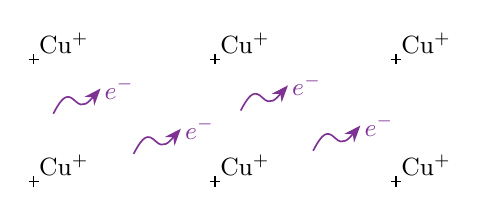
\begin{tikzpicture}
 \foreach \x in {0,2.3,4.6}{\foreach \y in {0,1.55}{\ioncu{\x}{\y}}}
 \electronlibre{.25}{.86}\electronlibre{1.27}{.35}
 \electronlibre{2.63}{.90}\electronlibre{3.55}{.39}
 \end{tikzpicture}}
\begin{document}
{\raggedright\fontsize{27}{31}\selectfont\bfseries Les conducteurs\par}
\planP{I}{sec:metal}
\planS{1}{sec:drude}
\planS{2}{sec:ohm}
\planSS{a}{sec:uniforme}
\planSS{b}{sec:lent}
\planSS{c}{sec:sinus}
\planS{3}{sec:cylindre}
\planS{4}{sec:joule}
\planP{II}{sec:maxwell}
\planS{1}{sec:gauss}
\planS{2}{sec:ampere}
\planS{3}{sec:bilan}
\planP{III}{sec:hall}
\planS{1}{sec:description}
\planS{2}{sec:classique}
\planP{IV}{sec:laplace}
\planS{1}{sec:rails}
\planS{2}{sec:interpretation}
\planS{3}{sec:definition}
\vspace{3mm}

On s'intéresse à la circulation du courant dans un fil pour comprendre ce qu'est le \textbf{courant}.

% Manuscrit, pages 1 à 3.
\section{Conduction électrique dans un métal}\label{sec:metal}
\subsection{Modèle de Drude}\label{sec:drude}
Dans cette partie, nous allons étudier la conduction électrique dans un conducteur. Pour ce faire,
nous adoptons le modèle de Drude : un métal comme le cuivre se modélise par un ensemble d'ions
positifs \(\mathrm{Cu}^{+}\) disposés régulièrement aux nœuds d'un réseau cristallin. Les ions
oscillent autour de leur position d'équilibre, mais ne peuvent pas se déplacer librement.
Ils sont immobiles en moyenne.

Chaque atome de cuivre a cédé un électron qui est libre de se déplacer dans le réseau cristallin.
Ces électrons subissent des interactions avec le réseau cristallin, avec lequel ils échangent de
l'énergie. L'énergie cinétique fournie par les électrons au réseau se retrouve souvent sous forme
de vibrations collectives du réseau (phonons). Le traitement classique du problème consiste à
considérer que les électrons subissent des chocs avec les ions positifs du réseau.
\deuxcol{.48}{\cuivreDrude}{%
\begin{itemize}
\item On étudie les interactions entre les électrons \(e^-\) et les ions \(\mathrm{Cu}^+\).
\item On néglige les interactions entre électrons.
\end{itemize}}

En l'absence de champ électrique imposé de l'extérieur, les électrons libres ont, à la suite
des différents chocs avec le réseau, des vitesses aléatoires. Il n'y a pas de déplacement
d'ensemble des électrons et il n'y a pas de courant.

On peut évaluer l'ordre de grandeur
de la vitesse quadratique moyenne des électrons en assimilant le \textbf{gaz d'électrons à un gaz parfait} :\label{verif:vitesse}
\[
 u=\sqrt{\av{v^2}}=\sqrt{\frac{3kT}{m}}.
\]
Au voisinage de \(300\unite K\), on obtient une vitesse \(u\) de l'ordre de \(100\unite{km\,s^{-1}}\).
La vitesse quadratique d'agitation thermique est considérable. Le libre parcours moyen d'un
électron entre deux chocs est de l'ordre de \(10^{-9}\unite m\).

L'application d'un champ électrique stationnaire entraîne un déplacement d'ensemble des électrons
sous l'effet de la force de Lorentz. Nous avons vu dans le premier chapitre que la vitesse de
déplacement d'ensemble des porteurs de charges mobiles, de l'ordre de quelques millimètres par
minute, est très faible devant la vitesse d'agitation thermique.

\begin{cadre}L'application d'un champ électrique stationnaire dans un
conducteur entraîne un déplacement d'ensemble des électrons dont la vitesse typique est
très faible devant la vitesse d'agitation thermique.\end{cadre}

\subsection{Loi d'Ohm locale}\label{sec:ohm}
\titr{Bilan des forces}
\begin{itemize}
\item Le champ électrique extérieur \(\E\) exerce une force sur l'électron.
\item Les chocs donnent lieu à une force due aux interactions entre les électrons \(e^-\) et les ions \(\mathrm{Cu}^+\).
\end{itemize}

Pour que le conducteur soit traversé par un courant électrique, il faut appliquer une tension
entre les deux extrémités du fil et donc créer dans le fil un champ électrique \(\E\).
Les charges \(q\) sont alors soumises à une force \(q\E\) qui devrait les accélérer. Or
l'expérience montre que, si l'on applique une tension \(U\) constante, l'intensité du courant et
donc la vitesse des charges sont constantes. Une force s'oppose donc à \(q\E\). Elle est due à
l'action du réseau métallique sur les électrons libres. Cette force peut être modélisée par une
force de frottement proportionnelle à la vitesse et de sens opposé :
\[
 -\frac m\tau\,\vv \qquad \text{(modélisation phénoménologique).}
\]

Cette force ne peut pas être assimilée à une force de frottement fluide comme celle rencontrée
dans le chapitre sur l'écoulement d'un fluide visqueux autour d'une sphère. Il s'agit d'une
force \emph{ad hoc} introduite pour rendre compte des observations et des interactions entre
les porteurs de charges mobiles et les porteurs de charges fixes. Ces forces n'ont pas la même
origine physique.

Cette force doit également être indépendante du référentiel. Dans un référentiel \((R)\) où le
conducteur serait en mouvement à la vitesse \(\vec V_C\) et l'électron à la vitesse \(\vv\),
la force s'écrirait
\[
 -\frac{m}{\tau}\,\vv'=-\frac{m}{\tau}\bigl(\vv-\vec V_C\bigr),
\]
où \(\vv'\) serait la \textbf{vitesse relative} des porteurs de charges libres par rapport aux porteurs liés.

Le vecteur vitesse envisagé ici est en fait la \textbf{vitesse moyenne} des électrons d'un volume
mésoscopique entourant l'électron considéré et non la vitesse totale d'un électron, composée de la
vitesse d'agitation thermique et de la vitesse due à la présence du champ électrique. Cela revient
à attribuer à un électron individuel la vitesse moyenne du volume mésoscopique autour de cet
électron, comme en mécanique des fluides.

Dans la suite du cours, nous prendrons les notations suivantes :
\begin{itemize}
\item \(q\) est la charge des porteurs de charges \textbf{libres} (électrons).
\item \(\vv\) est leur vitesse moyenne à l'échelle mésoscopique dans un référentiel d'étude
où le conducteur est au repos.
\item \(n\) est la densité volumique des porteurs de charges \textbf{mobiles}.
\item \(m\) est la masse d'un porteur de charge.
\end{itemize}
À l'échelle mésoscopique, \(\vv(M,t)\) et \(n(M,t)\) sont supposées uniformes.

% Manuscrit, pages 3 à 8.
\subsubsection{Dans un champ électrique uniforme et permanent}\label{sec:uniforme}
\textbf{Hypothèses :}
\begin{itemize}
\item Le champ électrique \(\E\) appliqué dans le conducteur est \textbf{permanent} et \textbf{uniforme}.
\item On effectue l'étude dans le référentiel où le conducteur est au repos.
\item On néglige le poids de l'électron.
\item On néglige les interactions entre électrons. Cela revient à négliger un terme lié à un
champ de pression dans le bilan des forces sur une particule fluide d'électrons.
\end{itemize}
\textbf{Système :} on considère une particule fluide d'électrons. C'est un système fermé.

Le théorème de la quantité de mouvement donne
\[
 nm\,\vol\,\frac{\mathrm D\vv}{\mathrm Dt}
   =(n\,\vol)\,q\E-\frac{m\vv}{\tau}\,(n\,\vol)
     \underbrace{-\grad P\,\vol}_{\substack{\text{terme négligé : interactions}\\
                                             \text{entre électrons négligées}}}.
\]
Il en résulte
\[
 m\left[\frac{\partial\vv}{\partial t}+
       \bigl(\vv\cdot\grad\bigr)\vv\right]
    =q\E-\frac{m\vv}{\tau}.
\]
Dans un champ \(\E\) uniforme, \(\vv\) est uniforme et
\(\bigl(\vv\cdot\grad\bigr)\vv=\vzero\). On obtient successivement
\begin{cadre}\[\frac{\partial\vv}{\partial t}+\frac{\vv}{\tau}=\frac{q\E}{m}.\]\end{cadre}
\begin{cadre}\[\vv(t)=\vec A\,e^{-t/\tau}+\frac{q\tau}{m}\E.\]\end{cadre}
Le vecteur \(\vec A\) est une constante d'intégration et \(\tau\) est le temps de relaxation.

Au bout d'un temps grand devant \(\tau\), la vitesse des porteurs de charge
\(\displaystyle\vv=\frac{q\tau}{m}\E\) est constante. La densité de courant s'écrit
\[
 \vj(M,t)=n(M,t)\,q\,\vv(M,t).
\]
Avec \(n(M,t)=n\) uniforme, on obtient
\bmath{\vj(M,t)=nq\,\vv(M,t).}
Expérimentalement, on constate que l'intensité du courant s'établit « instantanément ».
À l'échelle expérimentale, \(\tau\) est donc négligeable.
Ainsi, \(\displaystyle\vv=\frac{q\tau}{m}\E\) et on en déduit
\bmath{\vj=\frac{nq^2\tau}{m}\E.}

\begin{result}[5]
Le vecteur densité de courant est proportionnel à \(\E\) et de même sens :
\[
 \vj=\sigma_0\E,\qquad \sigma_0=\frac{nq^2\tau}{m}.
\]
La constante \(\sigma_0\), caractéristique du conducteur, est appelée \textbf{conductivité}.
Cette relation est appelée \textbf{loi d'Ohm locale}. Elle a été démontrée pour un
\textbf{champ électrique uniforme et permanent}, dans un \textbf{référentiel galiléen où le
conducteur est fixe}, \textbf{en l'absence de champ magnétique extérieur}.
\end{result}

\titr{Ordres de grandeur}
\begin{result}[5]Pour le cuivre, on mesure \(\displaystyle\sigma_0=6{,}2\times10^7\unite{S\,m^{-1}}\).\end{result}
D'après le cours sur les distributions de charges, \(n=8{,}5\times10^{28}\) électrons libres par mètre cube.

\textbf{Application numérique :}
\betoile{5}{\tau=2\times10^{-14}\unite s.}

\titr{Remarques}
\begin{itemize}
\item Dans le bilan des forces sur le porteur de charge, nous avons négligé la force de Lorentz
engendrée par le champ magnétique créé par le courant lui-même. On peut montrer que cette
composante magnétique est négligeable devant la composante électrique de la force de Lorentz.
\item Si l'on applique un champ magnétique extérieur \(\vB\), on ne peut plus négliger la
force de Lorentz \(q\vv\wedge\vB\) engendrée par ce champ. La loi d'Ohm précédente n'est
alors plus valable. Voir les exercices sur la \textbf{magnétorésistance} dans la feuille de TD.
\item Si le conducteur est mobile en présence d'un champ magnétique extérieur permanent \(\vB\),
la loi d'Ohm est remplacée par une loi d'Ohm généralisée de la forme
\[
 \vj(M,t)=\sigma_0\bigl(\E(M,t)+\vec U(M)\wedge\vB\bigr),
\]
où \(\vec U\) est la vitesse du conducteur au point considéré.
\end{itemize}

\subsubsection{Dans un champ électrique « lentement » variable dans le temps}\label{sec:lent}
Si le champ électrique appliqué reste uniforme et varie lentement dans le temps, la loi d'Ohm
précédente reste valable en champ électrique variable à condition que la durée caractéristique du
régime libre \(\vv=\vec A\,e^{-t/\tau}\) soit négligeable devant la durée caractéristique de
variation du champ électrique.

Pour un champ électrique non permanent, le temps caractéristique d'évolution du champ doit être
très supérieur à \(\tau\), de l'ordre de \(10^{-14}\unite s\) dans le cas du cuivre. Cette
hypothèse est peu contraignante.

Si le champ électrique n'est pas uniforme, il faut éventuellement tenir compte de l'accélération
convective des porteurs de charge. On suppose que ce terme est négligeable devant les autres
termes du théorème de la quantité de mouvement. Cette hypothèse revient à négliger les variations
spatiales du champ électrique sur l'échelle caractéristique de déplacement des porteurs de
charge. Dans ces conditions, la loi d'Ohm est encore valable pour un champ électrique dont le
temps caractéristique d'évolution est très supérieur à \(\tau\).

\titr{Ordres de grandeur}
\[
 \norme{(\vv\cdot\grad)\vv}\simeq\frac{v^2}{\lambda},
\]
où \(\lambda\) est la distance caractéristique de variation de \(\E\), et donc de \(\vv\).
De même,
\[
 \norme{\frac{\partial\vv}{\partial t}}\simeq\frac vT,
\]
où \(T\) est le temps caractéristique de variation de \(\E\), et donc de \(\vv\). Ainsi,
\[
 \frac{v^2}{\lambda}\ll\frac vT
 \quad\Longleftrightarrow\quad
 v\ll\frac{\lambda}{T}=c,\qquad c\ \text{étant la vitesse de la lumière}.
\]\label{verif:lambda}
On peut négliger l'accélération convective si \(v\) est très petite devant la vitesse de la
lumière. Or \(v\) est de l'ordre de quelques millimètres par minute : l'hypothèse est valable.

\begin{cadre}
Si les \textbf{fréquences du champ électrique sont très inférieures à \(1/\tau\)}, soit
\(10^{14}\unite{Hz}\) (fréquence du domaine optique) dans le cas du cuivre, on peut encore
écrire la loi d'Ohm locale sous la forme
\[
 \vj(M,t)=\sigma_0\E(M,t),\qquad \sigma_0=\frac{nq^2\tau}{m}.
\]
Les autres conditions de validité demeurent : l'étude est réalisée dans un \textbf{référentiel
galiléen où le conducteur est fixe}, \textbf{en l'absence de champ magnétique extérieur}.
\end{cadre}

\titr{Remarques}
\begin{itemize}
\item Lorsque l'on considère un champ électrique dépendant du temps, il y a également
nécessairement présence d'un champ magnétique dépendant du temps (cf. équations de Maxwell).\label{verif:variable}
Les effets des champs magnétiques induits par la présence d'un champ électrique dépendant
du temps peuvent en général être négligés pour la conduction électrique dans un métal.
Le rapport de la composante magnétique de la force de Lorentz à sa composante électrique est
d'autant plus faible que la vitesse des porteurs de charge est faible :
\[
 \frac{\norme{q\,\vv\wedge\vB}}{\norme{q\E}}\simeq\frac{vB}{E}.
\]
Dans le cas d'une onde électromagnétique, on peut montrer que l'ordre de grandeur du champ
magnétique est égal au rapport du champ électrique à la vitesse de la lumière.
Si les électrons sont non relativistes, c'est-à-dire si \(v\ll c\), la composante magnétique
associée à la variation temporelle du champ électrique est donc négligeable devant la
composante électrique de la force de Lorentz.
\item Un \textbf{conducteur parfait} est un conducteur ohmique dont la conductivité
\(\sigma_0\) est infinie. Ce modèle est souvent utilisé pour décrire simplement l'interaction
d'un métal avec une onde électromagnétique. Il correspond à une réalité expérimentale pour les
milieux supraconducteurs. La valeur \(\sigma_0=6{,}2\times10^7\unite{S\,m^{-1}}\) est déjà
assez grande.

Dans le modèle du conducteur parfait, la densité volumique de courant est toujours donnée
par \(\vj=\sigma_0\E\) et ne peut pas être infinie. Le champ électrique est donc nul
en tout point et à tout instant :
\bmath{\E(M,t)=\vzero,\qquad\forall M,\ \forall t.}
La conductivité \(\sigma_0\) étant infinie, le temps \(\tau\) l'est également : il n'y a
pas de force de frottement à introduire sur les porteurs de charge.
\end{itemize}

% Manuscrit, pages 8 à 10.
\subsubsection{Dans un champ électrique non uniforme et en régime sinusoïdal}\label{sec:sinus}
On suppose que le champ électrique varie sinusoïdalement dans le temps et l'on utilise la
notation complexe :
\[
 \cx{\E}(\vec r,t)=\cx{\E}(\vec r)\,e^{-\imag\omega t},
 \qquad
 \cx{\vv}(\vec r,t)=\cx{\vv}(\vec r)\,e^{-\imag\omega t}.
\]
\remaq la convention utilisée ici est celle de l'exponentielle \(e^{-\imag\omega t}\).

On néglige encore l'accélération convective des porteurs de charge. Cela revient à supposer que
la longueur d'onde associée à ce champ est très grande devant la distance parcourue par un
porteur de charge pendant une période, ce qui est raisonnable dès lors que les porteurs de charge
sont non relativistes.

On a toujours, cette fois en \textbf{régime sinusoïdal forcé},
\[
 \frac{\partial\vv}{\partial t}+\frac{\vv}{\tau}=\frac{q\E}{m}.
\]
Le principe fondamental de la dynamique appliqué à un porteur de charge donne une équation linéaire :
\[
 m\frac{\partial\vv}{\partial t}=q\E-\frac m\tau\,\vv.
\]
En un point \(M\) donné, on cherche donc des solutions sous la forme
\(\cx{\vv}=\cx{\vv}(\vec r)\,e^{-\imag\omega t}\) en \textbf{notation complexe}.
On en déduit
\[
 -\imag\omega\,\cx{\vv}=\frac qm\,\cx{\E}-\frac1\tau\,\cx{\vv},
 \qquad
 \cx{\vv}=\frac{q\tau}{m}\,\frac{1}{1-\imag\omega\tau}\,\cx{\E}.
\]
Ainsi,
\[
 \cx{\vj}=nq\,\cx{\vv}
   =\frac{nq^2\tau}{m}\,\frac{1}{1-\imag\omega\tau}\,\cx{\E}.
\]
\begin{cadre}
\[
 \cx{\vj}=\cx{\sigma}\,\cx{\E},\qquad
 \cx{\sigma}=\frac{nq^2\tau}{m}\,\frac{1}{1-\imag\omega\tau}
            =\frac{\sigma_0}{1-\imag\omega\tau}.
\]
La grandeur \(\sigma_0\) est la conductivité en régime permanent. L'étude a été réalisée dans un
\textbf{référentiel galiléen où le conducteur est fixe}, \textbf{en l'absence de champ magnétique
extérieur}.
\end{cadre}

\titr{Commentaires}
\begin{enumerate}[label=\arabic*)]
\item La loi d'Ohm porte maintenant sur des amplitudes complexes, comme pour l'impédance complexe \(\cx Z\).
\item Dans le cas d'une onde électromagnétique, il y a aussi un champ magnétique associé :
\[
 \cx{\vB}(\vec r,t)=\cx{\vB}(\vec r)\,e^{-\imag\omega t}.
\]
Pour une onde, l'ordre de grandeur est \(B(r)\simeq E(r)/c\). La partie magnétique de la force de
Lorentz est donc négligeable, comme dans la partie précédente, car les électrons sont non relativistes.
\item Il y a une différence de phase entre les variations du courant et celles du champ
si \(\partim(\cx{\sigma})\ne0\).
\item Lorsque \(\omega\tau\ll1\), ou \(\tau\ll1/\omega\), on a \(\cx{\sigma}\simeq\sigma_0\).
On retrouve ainsi les résultats du paragraphe b).
\item En présence d'un champ magnétique extérieur, la loi d'Ohm précédente n'est plus valable.
Voir l'exercice sur la magnétorésistance en régime variable du TD n\textsuperscript{o}~4.
\item Si la convention choisie pour les amplitudes complexes est \(e^{\imag\omega t}\),
l'expression de la conductivité complexe devient
\[
 \cx{\sigma}=\frac{\sigma_0}{1+\imag\omega\tau}.
\]
\item Dans les exercices en régime sinusoïdal forcé où la convention est imposée,
il faut faire attention aux signes.
\end{enumerate}

\subsection{Résistance d'un conducteur cylindrique}\label{sec:cylindre}
\noindent\begin{minipage}[c]{.585\linewidth}
On considère un conducteur ohmique cylindrique de section \(S\) et de longueur \(L\).
Entre ses deux extrémités \(A\) et \(B\), on applique une différence de potentiel
\(V_A-V_B\) \textbf{constante} (régime stationnaire).

On admet qu'il règne alors à l'intérieur du conducteur un champ électrique \(\E\) uniforme
et \textbf{parallèle aux génératrices du cylindre}.
\end{minipage}\hfill\begin{minipage}[c]{.39\linewidth}\centering
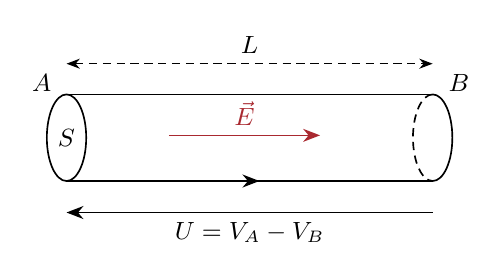
\begin{tikzpicture}
 \draw[semithick](0,-.55)--(4.65,-.55) (0,.55)--(4.65,.55);
 \draw[semithick](0,0)ellipse(.25 and .55);
 \draw[semithick](4.65,-.55)arc[start angle=-90,end angle=90,x radius=.25,y radius=.55];
 \draw[semithick,densely dashed](4.65,.55)arc[start angle=90,end angle=270,x radius=.25,y radius=.55];
 \node[pet]at(0,0){$S$};
 \node[above left,pet]at(-.13,.52){$A$}; \node[above right,pet]at(4.79,.52){$B$};
 \draw[cote,densely dashed](0,.94)--(4.65,.94) node[midway,above]{$L$};
 \draw[champ](1.30,.03)--(3.22,.03)node[midway,above]{$\E$};
 \draw[fleche](1.74,-.55)--(2.45,-.55);
 \draw[fleche](4.65,-.95)--(0,-.95)node[midway,below]{$U=V_A-V_B$};
\end{tikzpicture}
\end{minipage}\par
La tension aux bornes du conducteur est
\[
 U=V_A-V_B=\int_A^B\E\cdot\dd\vec\ell=E\,L .
\]
D'après la loi d'Ohm locale, l'intensité du courant dans le conducteur est
\(I=jS=\sigma_0 SE\). On peut éliminer \(E\) entre ces deux relations. On en déduit que la
tension \(\displaystyle U=\frac{L}{\sigma_0 S}I\) est proportionnelle à l'intensité du courant \(I\).
Le coefficient de proportionnalité est une constante caractéristique du conducteur appelée
\textbf{résistance}. En conclusion,
\betoile{4}{U=RI,\qquad R=\frac{L}{\sigma_0 S}=\rho_0\,\frac{L}{S}.}
La grandeur \(\rho_0=1/\sigma_0\) est appelée \textbf{résistivité} du conducteur.

Unités SI : \(\rho_0\) s'exprime en \(\mathrm{\Omega\,m}\) et \(\sigma_0\) en \(\mathrm{S\,m^{-1}}\).

% Manuscrit, pages 10 à 14.
\subsection{Effet Joule}\label{sec:joule}
Nous avons vu, dans le deuxième chapitre d'électromagnétisme, que le champ électromagnétique
fournit aux porteurs de charge une puissance volumique égale à
\[
 \densP=\vj\cdot\E.
\]

\titr{En régime permanent ou lentement variable}
Dans un conducteur ohmique en régime permanent ou lentement variable, \(\vj=\sigma_0\E\) et
\[
 \densP=\sigma_0\norme{\E}^2>0 .
\]
Le champ cède toujours de la puissance aux porteurs de charge. Cette énergie est ensuite cédée
au réseau cristallin au cours de chocs inélastiques. Le réseau cristallin cède à son tour cette
énergie à l'atmosphère par conduction thermique et par rayonnement : c'est l'effet Joule.

\textbf{Interprétation physique en régime stationnaire :} les porteurs de charge ont une vitesse
constante, moyennée sur un volume mésoscopique autour du porteur. Leur énergie cinétique ne
peut donc pas varier : ils doivent céder au matériau support la totalité de la puissance que
le champ électrique leur fournit. La force de friction assure le transfert d'énergie entre les
porteurs et le réseau cristallin. Celui-ci reçoit de l'énergie sous forme désordonnée : son
énergie interne et sa température augmentent. Lorsqu'un régime stationnaire thermique est
également établi, l'énergie interne du réseau ne peut plus augmenter. Le réseau transfère
alors son énergie à l'environnement extérieur par rayonnement ou par diffusion thermique.
\bmath{\densP=\sigma_0\norme{\E}^2=\frac{\norme{\vj}^2}{\sigma_0}.}

\titr{En régime sinusoïdal forcé à la pulsation \texorpdfstring{\(\omega\)}{ω}}
\deuxcol{.41}{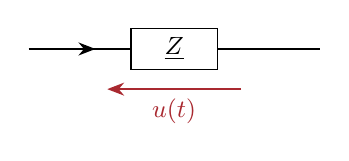
\begin{tikzpicture}
 \draw[semithick](-1.85,0)--(-.55,0) (.55,0)--(1.85,0);
 \draw[fleche](-1.66,0)--(-1.00,0);
 \draw[semithick](-.55,-.26)rectangle(.55,.26);\node at(0,0){$\cx Z$};
 \draw[champ](.85,-.51)--(-.85,-.51)node[midway,below]{$u(t)$};
\end{tikzpicture}}{On considère un dipôle passif linéaire d'impédance \(\cx Z\).}
On a \(\cx u=\cx Z\,\cx i\), avec
\[
 \left\{\begin{aligned}
 u(t)&=U\cos(\omega t+\varphi_u),\\
 i(t)&=I\cos(\omega t+\varphi_i).
 \end{aligned}\right.
\]
La puissance instantanée \textbf{reçue} par le dipôle est \(p(t)=u(t)i(t)\). On a donc
\[
 p(t)=UI\cos(\omega t+\varphi_u)\cos(\omega t+\varphi_i).
\]
\begin{cadre}
\[
 p(t)=\underbrace{\frac{UI}{2}\cos(2\omega t+\varphi_u+\varphi_i)}
                        _{\text{grandeur sinusoïdale à }2\omega}
        +\underbrace{\frac{UI}{2}\cos(\varphi_u-\varphi_i)}_{\av{p}}.
\]
\end{cadre}
\textbf{Attention :} \(\cx p(t)\ne\cx u(t)\,\cx i(t)\). Il ne faut \textbf{jamais}
multiplier deux amplitudes complexes.\label{verif:produit}

\deuxcol{.47}{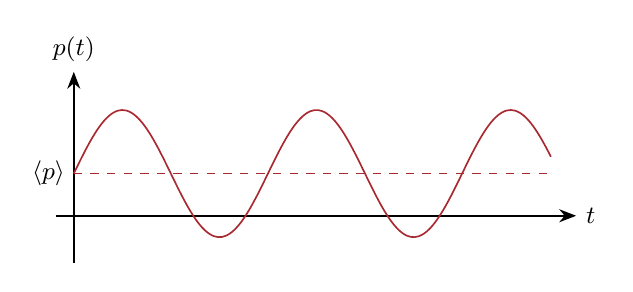
\begin{tikzpicture}[x=1cm,y=.85cm]
 \draw[fleche](-.23,0)--(6.38,0)node[right]{$t$};
 \draw[fleche](0,-.70)--(0,2.15)node[above]{$p(t)$};
 \draw[rougechamp,dashed](0,.63)--(6.06,.63);
 \draw[rougechamp,semithick,domain=0:6.06,samples=120,smooth] plot(\x,{.63+.95*sin(146*\x)});
 \node[left,pet]at(-.05,.63){$\av p$};
\end{tikzpicture}}{En régime sinusoïdal forcé,
\bmath{\av{p(t)}=\frac{UI}{2}\cos(\varphi_u-\varphi_i).}}

\Needspace{9\baselineskip}
\begin{result}[5]
\textbf{Puissance complexe :}\label{verif:conjugue}
\[
 \cx p=\frac12\,\cx u\,\cx i^{*}
 \qquad\text{ou}\qquad
 \frac12\,\cx i\,\cx u^{*}.
\]
\end{result}
On obtient
\begin{align*}
 \partre(\cx p)
 &=\partre\!\left(\frac12\,Ue^{\imag(\omega t+\varphi_u)}
                        I e^{-\imag(\omega t+\varphi_i)}\right)\\
 &=\partre\!\left(\frac12\,UIe^{\imag(\varphi_u-\varphi_i)}\right)
  =\frac12\,UI\cos(\varphi_u-\varphi_i).
\end{align*}
\label{verif:expo}
\betoile{4}{\av{p(t)}=\partre(\cx p).}

\begin{exemple}
\examtitle{Exemples}
\begin{align*}
 \av{p(t)}&=\partre\!\left(\tfrac12\,\cx u\,\cx i^{*}\right)
 =\partre\!\left(\tfrac12\,\cx Z\,\cx i\,\cx i^{*}\right).
\end{align*}
\bmath{\av{p(t)}=\frac12 I^2\partre(\cx Z).}
\fig{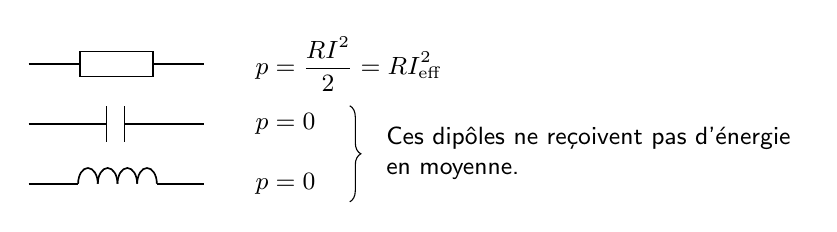
\begin{tikzpicture}[x=1cm,y=1cm]
 % Résistance, condensateur et bobine idéaux.
 \draw[semithick](0,0)--(.65,0) (1.58,0)--(2.23,0);
 \draw[semithick](.65,-.16)rectangle(1.58,.16);
 \draw[semithick](0,-.76)--(.99,-.76) (1.22,-.76)--(2.23,-.76);
 \draw[semithick](.99,-.99)--(.99,-.53) (1.22,-.99)--(1.22,-.53);
 \draw[semithick](0,-1.52)--(.63,-1.52);
 \foreach \x in {.63,.88,1.13,1.38}{
   \draw[semithick] (\x,-1.52) arc[start angle=180,end angle=0,x radius=.125,y radius=.20];}
 \draw[semithick](1.63,-1.52)--(2.23,-1.52);
 \node[anchor=west]at(2.76,0){$\displaystyle p=\frac{RI^2}{2}=RI_{\mathrm{eff}}^2$};
 \node[anchor=west]at(2.76,-.76){$p=0$};\node[anchor=west]at(2.76,-1.52){$p=0$};
 \draw[decorate,decoration={brace,amplitude=4pt}](4.08,-.53)--(4.08,-1.75);
 \node[anchor=west,align=left,text width=5.25cm] at(4.42,-1.13)
 {Ces dipôles ne reçoivent pas d'énergie en moyenne.};
\end{tikzpicture}}
\end{exemple}

\titr{Généralisation}
En régime sinusoïdal forcé à la pulsation \(\omega\), on a
\begin{align*}
 \av{\vj\cdot\E}
  &=\partre\!\left(\tfrac12\,\cx{\vj}\cdot\cx{\E}^{*}\right),&
 \av{\frac{\E\wedge\vB}{\mu_0}}
  &=\partre\!\left(\frac{\cx{\E}\wedge\cx{\vB}^{*}}{2\mu_0}\right),\\[3pt]
 \av{\tfrac12\eps E^2}
  &=\partre\!\left(\tfrac14\eps\,\cx{\E}\cdot\cx{\E}^{*}\right),&
 \av{\frac{B^2}{2\mu_0}}
  &=\partre\!\left(\frac{1}{4\mu_0}\,\cx{\vB}\cdot\cx{\vB}^{*}\right).
\end{align*}
Dans le cas général, on montre que la puissance \textbf{moyenne} volumique donnée aux
porteurs de charge se calcule à l'aide des amplitudes complexes du champ électrique et du
vecteur densité de courant :
\[
 \av{\densP}=\av{\vj\cdot\E}
  =\frac12\partre\bigl(\cx{\vj}\cdot\cx{\E}^{*}\bigr)
  =\frac12\partre\!\left(\cx{\sigma}\,\norme{\cx{\E}}^2\right)\ne0 .
\]
La puissance absorbée en moyenne par les porteurs de charge est non nulle.

Lorsque \(\omega\tau\ll1\), \(\cx{\sigma}=\sigma_0\). La puissance absorbée en moyenne par
les porteurs de charge est positive et de l'énergie est dissipée par effet Joule en moyenne.

Lorsque \(\omega\tau\gg1\), on a \(\displaystyle\cx{\sigma}=\imag\,\frac{nq^2}{m\omega}\).
La conductivité complexe est imaginaire pure. Le vecteur densité de courant et le champ
électrique varient sinusoïdalement en quadrature. Pour \(\omega\tau\gg1\),
\(\partre\bigl(\cx{\vj}\cdot\cx{\E}^{*}\bigr)=0\) et aucune énergie n'est dissipée par
effet Joule \textbf{en moyenne}. La puissance moyenne fournie par le champ électrique aux
conducteurs de charges est alors nulle.\label{verif:joule}

% Manuscrit, pages 14 à 17.
\Needspace{11\baselineskip}
\section{Équations de Maxwell dans un conducteur ohmique}\label{sec:maxwell}
\subsection{Utilisation de l'équation de Maxwell-Gauss}\label{sec:gauss}
\titr{Régime « lentement » variable}
Nous allons montrer que la densité volumique de charge à l'intérieur d'un conducteur ohmique
est nulle tant que le régime d'évolution du champ électromagnétique n'est pas trop rapide.

On suppose ici que l'on peut écrire la loi d'Ohm locale en grandeurs réelles :
\(\vj=\sigma_0\E\). Pour le cuivre, cela signifie que les champs électriques appliqués ont
des fréquences très inférieures à \(10^{14}\unite{Hz}\).

L'équation locale de conservation de la charge s'écrit
\(\displaystyle \frac{\partial\rho}{\partial t}+\divg(\vj)=0
 =\frac{\partial\rho}{\partial t}+\divg(\sigma_0\E)\).
On suppose le conducteur homogène : \(\sigma_0\) est constante dans tout le conducteur. Ainsi, \(\displaystyle \frac{\partial\rho}{\partial t}+\sigma_0\divg(\E)=0\).
En réinjectant l'équation de Maxwell-Gauss, il vient
\(\displaystyle \frac{\partial\rho}{\partial t}+\frac{\sigma_0\rho}{\eps}=0\), soit
\bmath{\frac{\partial\rho}{\partial t}+\frac{\rho}{\tau'}=0,
       \qquad \tau'=\frac{\eps}{\sigma_0}.}
\bmath{\rho(M,t)=\rho(M,t_0)\,e^{-(t-t_0)/\tau'}.}

Lorsque, pour une raison quelconque, on engendre localement un excédent de charges se traduisant
par une densité volumique \(\rho(M,t_0)\), cet excédent disparaît sur une durée de quelques
\(\tau'\). Le milieu redevient ainsi localement neutre : \(\rho(M,t_0)=0\).\label{verif:instant}

\begin{cadre}
La densité volumique de charge à l'intérieur d'un conducteur ohmique est toujours nulle si le
temps caractéristique d'évolution du champ électromagnétique est très supérieur à
\(\displaystyle\tau'=\frac{\eps}{\sigma_0}\).
\end{cadre}

\titr{Valeurs numériques pour le cuivre et conséquences}
\textbf{Application numérique :} \(\tau'\simeq10^{-19}\unite s\).

On se place en régime lentement variable : \(T\gg\tau=10^{-14}\unite s\). On a
\(\rho=0\) sur un temps \(\tau'=10^{-19}\unite s\ll\tau\). On a donc \(T\gg\tau'\) :
en régime lentement variable, on peut écrire
\bmath{\rho(M,t)=0.}

\remaq dans le cas d'un conducteur parfait, \(\tau'=\eps/\sigma_0=0\). Ainsi, \(\rho=0\) :
la densité volumique de charge est nulle à tout instant et en tout point du conducteur.

\remaq il peut y avoir des charges sur la surface.
\deuxcol{.42}{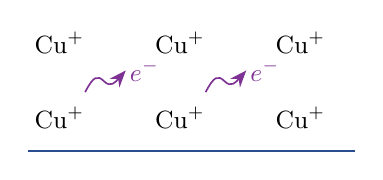
\begin{tikzpicture}[scale=.86]
 \draw[bleurep](-.46,-.49)--(4.36,-.49);
 \foreach \x in {0,1.78,3.56}{\foreach \y in {0,1.11}{
 \node[pet] at(\x,\y){$\mathrm{Cu}^+$};}}
 \electronlibre{.38}{.38}\electronlibre{2.16}{.38}
\end{tikzpicture}}{Le courant et la neutralité électrique coexistent :
\(\vj=\sigma_0\E\) et \(\rho=0\).}

\titr{Régime sinusoïdal forcé quelconque}
Reprenons l'étude précédente en supposant maintenant que le champ électrique et le vecteur
densité de courant sont liés par la relation suivante en grandeurs complexes :
\(\displaystyle \cx{\vj}=\frac{\sigma_0}{1-\imag\omega\tau}\,\cx{\E}\).
En grandeurs complexes, la loi de conservation de la charge devient
\(\displaystyle \frac{\partial\cx{\rho}}{\partial t}+\divg(\cx{\vj})=0
 =-\imag\omega\,\cx{\rho}+\divg(\cx{\sigma}\,\cx{\E})\).
En supposant à nouveau la conductivité \(\cx{\sigma}\) uniforme, il vient
\[
 -\imag\omega\,\cx{\rho}+\cx{\sigma}\divg(\cx{\E})
  =-\imag\omega\,\cx{\rho}+\cx{\sigma}\,\frac{\cx{\rho}}{\eps}
  =0=\cx{\rho}\left(-\imag\omega+\frac{\cx{\sigma}}{\eps}\right).
\]
On en déduit également que la densité volumique de charge est nulle en général.

\Needspace{9\baselineskip}
\subsection{Équation de Maxwell-Ampère}\label{sec:ampere}
\deuxcol{.40}{\(\displaystyle
 \rot(\vB)=\mu_0\vj+\frac1{c^2}\frac{\partial\E}{\partial t}.\)}{%
On considère une évolution temporelle sinusoïdale du champ électrique :
\(\cx{\E}(M,t)=\cx{\vec E_0}(M)\,e^{-\imag\omega t}\).}
On cherche à montrer que \(\displaystyle \mu_0 j\gg\frac1{c^2}\norme{\frac{\partial\E}{\partial t}}\).
Les inégalités successives s'écrivent
\[
\begin{aligned}
 \mu_0 j\gg\frac1{c^2}\norme{\frac{\partial\E}{\partial t}}
 &\ \Longleftrightarrow\
 \mu_0\module{\frac{\sigma_0}{1+\imag\omega\tau}}E \gg\frac1{c^2}\,\omega E
 &&\ \Longleftrightarrow\
   \frac{c^2\mu_0\sigma_0}{\module{1+\imag\omega\tau}\,\omega}\gg1\\[2pt]
 &\ \Longleftrightarrow\
   \frac{\omega\module{1+\imag\omega\tau}\eps}{\sigma_0}\ll1
 &&\ \Longleftrightarrow\
   \omega\tau'\module{1+\imag\omega\tau}\ll1 .
\end{aligned}
\]
Si \(\omega\tau\ll1\), la condition est vérifiée : on a automatiquement \(\omega\tau'\ll1\),
car \(\tau'\sim10^{-5}\tau\). Il faut donc
\bmath{f\ll10^{14}\unite{Hz}.}
\titr{Conclusion}
\begin{cadre}
Le courant de déplacement \textbf{à l'intérieur d'un bon conducteur} est toujours négligeable
devant la densité volumique de courant tant que la fréquence caractérisant l'évolution du champ
électromagnétique est très inférieure à \(10^{14}\unite{Hz}\).
\end{cadre}
\begin{cadre}
Dans le modèle du conducteur parfait, on peut toujours négliger le courant de déplacement
devant la densité volumique de courant à l'intérieur du conducteur.
\end{cadre}
\titr{Conséquence}
\bmath{\rot(\vB)=\mu_0\vj.}
Il en résulte que \(\divg\bigl(\rot(\vB)\bigr)=\mu_0\divg(\vj)=0\).
\begin{cadre}
\(\divg(\vj)=0\). Dans un bon conducteur ohmique, le vecteur densité de courant est à flux
conservatif. La loi des nœuds est donc valable.
\end{cadre}

% Le manuscrit réemploie « II.2 » pour le bilan qui suit le paragraphe II.2.
\subsection{Bilan}\label{sec:bilan}
\begingroup
\renewcommand{\arraystretch}{1.10}\setlength{\tabcolsep}{7pt}
\newcommand{\casebilan}[1]{\begin{minipage}[t]{\linewidth}\centering
\vspace{1.5pt}#1\par\vspace{1.5pt}\end{minipage}}
\noindent\begin{tabularx}{\linewidth}{|X|X|}
\hline
\casebilan{\textbf{Régime « lentement » variable}\\[2pt]\(f\ll10^{14}\unite{Hz}\)}
&
\casebilan{\textbf{Régime sinusoïdal forcé à \(\omega\)}\\[2pt]Fréquence \(f\) quelconque}\\ \hline
\casebilan{\(\vj=\sigma_0\E\)\\[4pt]\(\rho=0\)}
&
\casebilan{\(\displaystyle\cx{\vj}=\cx{\sigma}\,\cx{\E},\quad
 \cx{\sigma}=\frac{\sigma_0}{1\mp\imag\omega\tau}\)\\[4pt]\(\rho=0\)}\\ \hline
\casebilan{\(\displaystyle\divg\E=0,\qquad \rot\E=-\frac{\partial\vB}{\partial t}\)\\[6pt]
 \(\displaystyle\rot\vB=\mu_0\vj,\qquad\divg\vB=0\)}
&
\casebilan{\(\displaystyle\divg\E=0,\qquad\rot\E=-\frac{\partial\vB}{\partial t}\)\\[6pt]
 \(\displaystyle\rot\vB=\mu_0\vj+\frac1{c^2}\frac{\partial\E}{\partial t},\qquad\divg\vB=0\)\\[5pt]
 \(\displaystyle\rot\cx{\vB}
 =\mu_0\cx{\sigma}\,\cx{\E}-\frac{\imag\omega}{c^2}\cx{\E}\)}\\ \hline
\casebilan{La loi des nœuds est valable.\\
 Le vecteur \(\vj\) est à flux conservatif.}
&\\ \hline
\end{tabularx}\par
\endgroup

% Manuscrit, pages 17 à 20.
\Needspace{11\baselineskip}
\section{L'effet Hall}\label{sec:hall}
\subsection{Description}\label{sec:description}
\deuxcol{.44}{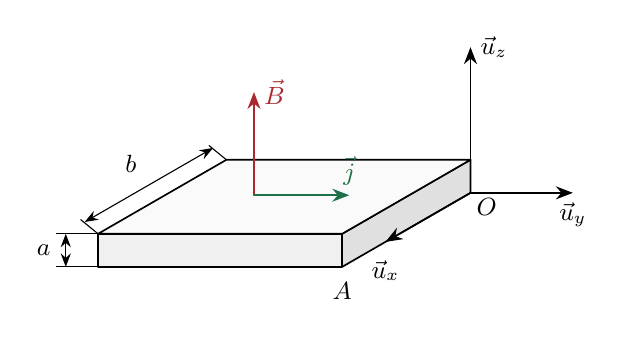
\begin{tikzpicture}[line join=round,line cap=round]
  % L'origine O est sur la face arrière ; OA suit la direction positive de x.
  \coordinate (O) at (0,0); \coordinate (A) at (-1.63,-.94);
  \coordinate (C) at (-3.10,0); \coordinate (D) at (-4.73,-.94);
  \coordinate (Ot) at (0,.42); \coordinate (At) at (-1.63,-.52);
  \coordinate (Ct) at (-3.10,.42); \coordinate (Dt) at (-4.73,-.52);
  \draw[semithick,fill=black!6] (Dt)--(At)--(A)--(D)--cycle;
  \draw[semithick,fill=black!12] (At)--(Ot)--(O)--(A)--cycle;
  \draw[semithick,fill=black!2] (Dt)--(Ct)--(Ot)--(At)--cycle;
  \draw[fleche] (O)--(1.30,0) node[below] {$\uy$};
  \draw[fleche] (O)--(0,1.85) node[right] {$\uz$};
  \draw[fleche] (O)--(-1.08,-.623) node[below=3pt] {$\ux$};
  \node[below right,inner sep=2pt] at (O) {$O$};
  \node[below=2pt] at (A) {$A$};
  \coordinate (H) at (-2.75,-.03);
  \draw[champ] (H)--++(0,1.31) node[right,rougechamp] {$\vB$};
  \draw[courant] (H)--++(1.21,0) node[above,vertcour] {$\vj$};
  \draw[thin] (D)--++(-.53,0) (Dt)--++(-.53,0);
  \draw[cote] ($(D)+(-.41,0)$)--node[left=2pt] {$a$}($(Dt)+(-.41,0)$);
  \draw[thin] (Ct)--++(-.22,.18) (Dt)--++(-.22,.18);
  \draw[cote] ($(Dt)+(-.17,.15)$)--node[above left=1pt] {$b$}($(Ct)+(-.17,.15)$);
\end{tikzpicture}}{Un morceau de métal, en cuivre par exemple, de section droite rectangulaire située dans le plan
\((\ux,\uz)\), est parcouru par un courant constant de densité
\(\displaystyle\vj=\frac I{ab}\uy\) et placé dans un champ magnétique
\(\vB=B\uz\), avec \(B>0\).}

Expérimentalement, on constate qu'une différence de potentiel \(V_A-V_O=\UH\) apparaît entre
les deux faces parallèles au plan \((\vB,\vj)\). Son signe dépend de la nature du conducteur.
Sa valeur est proportionnelle à l'intensité \(I\) du courant et à \(B\), et inversement
proportionnelle à l'épaisseur \(a\) du conducteur :
\begin{cadre}
\textbf{Tension de Hall :}
\[
 \UH=\RH\,\frac{IB}{a}.
\]
\end{cadre}
\(\RH\) est une constante caractéristique du métal, appelée \textbf{constante de Hall}.
Pour le cuivre, \(\RH=0{,}5\times10^{-10}\) en unités SI.\label{verif:cuivre}

\subsection{Modélisation classique}\label{sec:classique}
Au moment de l'établissement du champ magnétique \(\vB\), un porteur de charge est soumis
à la force de Lorentz
\(\displaystyle\vec F=q\vv\wedge\vB=\frac{\vj}{n}\wedge\vB\).
Il est donc dévié parallèlement à \(\ux\) et dans le sens de \(\ux\), quel que soit le signe de \(q\).

Des porteurs de charge s'accumulent ainsi progressivement sur la face \(x=b\), créant un champ
électrique, le \textbf{champ de Hall} \(\EH=E_{\mathrm H}\ux\). Sa valeur croît au cours du temps et son sens
dépend du signe de \(q\) : si \(q<0\), alors \(E_{\mathrm H}>0\).

\Needspace{6\baselineskip}
Les charges assurant le passage du courant électrique sont alors soumises à deux forces :
\begin{itemize}
\item la force électrique \(q\EH\) ;
\item la force magnétique \(q\vv\wedge\vB\).
\end{itemize}
Ces forces sont parallèles à \(\ux\) et de sens opposés. La déviation des porteurs de charge
diminue à mesure que \(E_{\mathrm H}\) augmente. Elle s'annule lorsque
\(q\EH=-q\vv\wedge\vB\), soit
\bmath{\EH=-\vv\wedge\vB.}
On a \(\vv=v\uy\), avec \(v<0\) si \(q<0\), d'où
\(\EH=-vB\uy\wedge\uz=-vB\ux\).

La différence de potentiel \(V_A-V_O=\UH\) entre le point \(A\), défini par
\(\fle{OA}=b\ux\), et l'origine \(O\) se déduit de la circulation du champ :
\begin{align*}
 \int_O^A\EH\cdot\dd\vec M&=V(O)-V(A)=-\UH,\\
 \UH&=-\int_0^b E_{\mathrm H,x}\,\dd x
      =\int_0^b vB\,\dd x .
\end{align*}\label{verif:hallint}
On obtient ainsi \(\UH=vBb\). Or \(I=jS\) et \(j=nqv\).\label{verif:hallj} D'où
\(\displaystyle \UH=\frac{j}{nq}Bb=\frac{IBb}{nqS}\), soit
\bmath{V_A-V_O=\UH=\frac{1}{nq}\frac{IB}{a}.}

Conformément aux résultats expérimentaux, ce modèle prévoit une tension de Hall proportionnelle
à \(IB/a\). Il prévoit aussi la valeur de la constante de Hall :
\bmath{\RH=\frac{1}{n\module q}.}
Le signe de \(\RH\) dépend du signe de \(q\). Dans la plupart des métaux, on trouve
\(\RH<0\).\label{verif:hallr}
\begin{exemple}
\examtitle{Exemple}
Pour le cuivre, calculer la valeur théorique de \(\RH\).

\textbf{Application numérique :} \(\RH\simeq10^{-11}\) en unités SI.
\end{exemple}
L'accord entre l'expérience et le modèle n'est pas trop mauvais, mais il n'est pas parfait.
Ce modèle théorique prévoit en particulier une tension \(V_A-V_O=\UH\) du signe des charges.
Expérimentalement, on constate qu'elle est bien négative pour la plupart des métaux, mais
\textbf{positive pour quelques-uns}.

À basse température et pour des champs élevés, la tension de Hall n'est plus proportionnelle
à \(IB/a\). La mécanique classique est rarement un outil parfait pour étudier l'atome ;
la mécanique quantique est le plus souvent indispensable.

L'effet Hall est appliqué à la mesure des champs magnétiques. Si l'on utilise comme matériau
un métal tel que le cuivre, \(\RH\approx10^{-10}\) en unités SI. Or
\(\displaystyle\UH=\RH\frac{IB}{a}=\RH jbB\).
Les valeurs maximales des tensions de Hall obtenues avec un ruban métallique sont de l'ordre
du \(\mu\mathrm V\) pour un champ magnétique élevé, de l'ordre du tesla, et avec des rubans
plats qui maximisent la tension de Hall (petites valeurs de \(a\)).

Il est donc indispensable de disposer d'un matériau dans lequel \(\RH\) serait plus grand.
La charge \(q\) d'un porteur ne peut pas diminuer. C'est donc le \textbf{nombre de porteurs
de charge par unité de volume} qui doit être beaucoup plus faible. Ces matériaux existent :
ce sont les \textbf{semi-conducteurs}. Dans les semi-conducteurs, on peut obtenir des densités
de porteurs de charge de l'ordre de \(10^{22}\unite{m^{-3}}\). Pour ces matériaux, le modèle
précédent est trop simpliste, car il y a deux types de porteurs de charge : les électrons et
les trous. Dans les \textbf{sondes à effet Hall}, on utilise des semi-conducteurs, comme
l'arséniure de gallium \(\mathrm{AsGa}\), et l'on peut obtenir des tensions de l'ordre du
\(\mathrm{mV}\).

% Manuscrit, pages 20 et 21.
\section{La force de Laplace}\label{sec:laplace}
\subsection{Mise en évidence expérimentale}\label{sec:rails}
\deuxcol{.48}{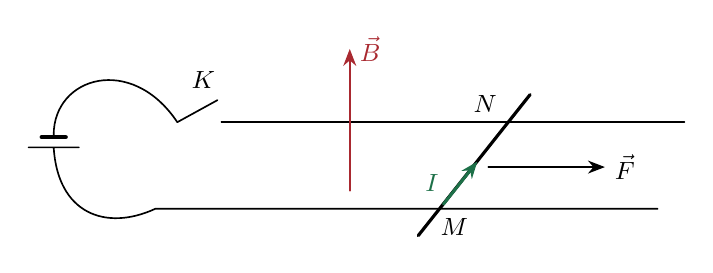
\begin{tikzpicture}[line join=round,line cap=round]
  % Deux rails horizontaux en perspective et leur circuit d'alimentation.
  \draw[semithick] (-2.6,.62)..controls(-3.18,1.49) and(-4.17,1.20)..(-4.17,.46);
  \draw[line width=1.7pt] (-4.32,.43)--(-4.02,.43);
  \draw[semithick] (-4.49,.30)--(-3.85,.30) (-4.17,.30)
    ..controls(-4.12,-.54) and(-3.51,-.77)..(-2.88,-.48)--(3.5,-.48);
  \draw[semithick] (-2.60,.62)--(-2.09,.90);
  \draw[semithick] (-2.04,.62)--(3.84,.62);
  \node[above=1pt] at (-2.27,.89) {$K$};
  \draw[line width=1.15pt] (.46,-.82)--(1.88,.97);
  \node[below right] at (.62,-.48) {$M$};
  \node[above left] at (1.58,.62) {$N$};
  \draw[courant,line width=1.1pt] (.78,-.42)--(1.21,.12)
    node[midway,left=4pt] {$I$};
  \draw[champ] (-.41,-.25)--(-.41,1.55) node[right] {$\vB$};
  \draw[fleche] (1.35,.05)--(2.83,.05) node[right] {$\vec F$};
\end{tikzpicture}}{Un barreau métallique \(MN\) est mobile sur deux rails horizontaux. Un générateur de courant
continu permet de faire passer un courant \(I\) dans les rails et le barreau. Le barreau est
placé dans le champ magnétique \(\vB\), vertical, créé par un aimant. À la fermeture de
l'interrupteur \(K\), on constate que le barreau se déplace parallèlement aux rails.
Le sens de son mouvement dépend du sens du courant et de celui du champ magnétique.}

\subsection{Interprétation}\label{sec:interpretation}
\deuxcol{.31}{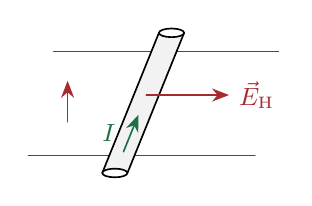
\begin{tikzpicture}[line cap=round,line join=round]
  \draw[bleurep,thin] (-1.5,.06)--(1.38,.06) (-1.18,1.38)--(1.68,1.38);
  \coordinate (b) at (-.40,-.16); \coordinate (h) at (.32,1.62);
  \fill[black!5] ($(b)+(-.16,0)$)--($(h)+(-.16,0)$)--($(h)+(.16,0)$)--($(b)+(.16,0)$)--cycle;
  \draw[semithick] ($(b)+(-.16,0)$)--($(h)+(-.16,0)$) ($(b)+(.16,0)$)--($(h)+(.16,0)$);
  \draw[semithick,fill=white] (b) ellipse[x radius=.16,y radius=.055];
  \draw[semithick,fill=white] (h) ellipse[x radius=.16,y radius=.055];
  \draw[courant] (-.29,.11)--(-.10,.58) node[midway,left=2pt] {$I$};
  \draw[champ] (0,.83)--(1.05,.83) node[right] {$\EH$};
  \draw[champ] (-1.0,.49)--(-1.0,1.01);
\end{tikzpicture}}{Soit un élément de conducteur cylindrique de longueur \(L\), parcouru par un
courant continu \(I\) et placé dans un champ magnétique \(\vB\).}

Les porteurs de charge, soumis à la force de Lorentz \(\vec F=q\vv\wedge\vB\), créent en
régime permanent le champ de Hall \(\EH=-\vv\wedge\vB\). Pour l'électron, \(q=-e\).

Le réseau métallique fixe porte une charge par unité de volume \(-nq\) : les ions ont pour charge
\(-q=+e\). Placé dans le champ \(\EH\), le réseau est soumis à une \textbf{force électrostatique
par unité de volume} :
\bmath{-nq\EH=+nq\vv\wedge\vB=\vj\wedge\vB.}
Un volume \(\vol\) du conducteur subit donc la force
\betoile{5}{\dd^3\vec F=\vj\wedge\vB\,\vol.}
Le conducteur étant cylindrique, de longueur \(L\) et de section \(S\), il est soumis à la force
\[
 \vec F=\iiint\vj\wedge\vB\,\vol
       =S L\,\vj\wedge\vB=S j\,\vec L\wedge\vB=I\vec L\wedge\vB,
       \qquad \text{appelée \textbf{force de Laplace} :}
\]
\bmath{\vec F=I\vec L\wedge\vB.}
\(\vec L\) est le vecteur de norme \(L\), parallèle au vecteur densité de courant \(\vj\)
et de même sens.

\subsection{Application : ancienne définition légale de l'ampère}\label{sec:definition}
\noindent\begin{minipage}[c]{.69\linewidth}
Un fil rectiligne supposé infini, parcouru par un courant \(I_1\), crée en un point distant
de \(d\) un champ magnétique \(\vB\) de valeur \(\displaystyle B=\frac{\mu_0}{2\pi}\frac{I_1}{d}\).
Si un deuxième fil rectiligne et infini, parcouru par un courant \(I_2\), est placé
parallèlement au premier, il est soumis à une force de Laplace.

Chaque longueur \(L\) du conducteur 2 est soumise à la force \(\vec F=I_2\vec L\wedge\vB\).
Or \(\vB\) est perpendiculaire à \(\vec L\), donc
\[
 F=I_2LB=\frac{\mu_0}{2\pi}\frac{I_1I_2}{d}L .
\]
Cette force est attractive si \(I_1\) et \(I_2\) sont de même sens et répulsive dans le cas
contraire.
\end{minipage}\hfill\begin{minipage}[c]{.28\linewidth}\centering
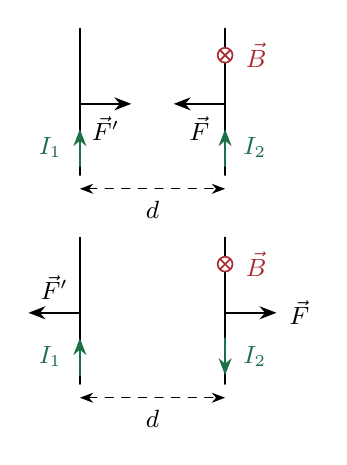
\begin{tikzpicture}[line cap=round,scale=.87]
  \foreach \h/\cas in {0/1,-3.05/-1}{
    \begin{scope}[yshift=\h cm]
      \draw[semithick] (0,0)--(0,2.14) (2.12,0)--(2.12,2.14);
      \draw[courant] (0,.13)--(0,.67) node[midway,left=3pt] {$I_1$};
      \ifnum\cas=1
        \draw[courant] (2.12,.13)--(2.12,.67) node[midway,right=3pt] {$I_2$};
        \draw[fleche] (0,1.04)--(.75,1.04) node[midway,below=1pt] {$\vec F'$};
        \draw[fleche] (2.12,1.04)--(1.37,1.04) node[midway,below=1pt] {$\vec F$};
      \else
        \draw[courant] (2.12,.67)--(2.12,.13) node[midway,right=3pt] {$I_2$};
        \draw[fleche] (0,1.04)--(-.75,1.04) node[midway,above=1pt] {$\vec F'$};
        \draw[fleche] (2.12,1.04)--(2.87,1.04) node[right=1pt] {$\vec F$};
      \fi
      \draw[rougechamp,fill=white,semithick] (2.12,1.75) circle[radius=.108];
      \draw[rougechamp,semithick] (2.045,1.675)--(2.195,1.825) (2.045,1.825)--(2.195,1.675);
      \node[right=4pt,rougechamp] at (2.12,1.75) {$\vB$};
      \draw[cote,dashed] (0,-.20)--node[below=1pt] {$d$}(2.12,-.20);
    \end{scope}}
\end{tikzpicture}
\end{minipage}\par
\Needspace{9\baselineskip}
En 1948, lors de la 9\textsuperscript{e} Conférence générale des poids et mesures, l'ampère
est adopté comme unité de base aux côtés du mètre, du kilogramme et de la seconde : ces unités
constituent le système MKSA.
\begin{cadre}
\textbf{L'ampère est l'intensité d'un courant constant qui, maintenu dans deux fils rectilignes,
parallèles et de longueur infinie, distants de \(1\unite m\) l'un de l'autre dans le vide,
produirait entre ces conducteurs une force égale à \(2\times10^{-7}\unite N\) par mètre de
longueur.}
\end{cadre}

Cette définition, restée en vigueur jusqu'au 20 mai 2019, donnait à la perméabilité magnétique
du vide \(\mu_0\) la valeur de \(4\pi\times10^{-7}\) en unités SI. Elle fixait aussi toutes
les unités qui en dépendent, en particulier le volt, le coulomb et le tesla.

Lors de la 26\textsuperscript{e} Conférence générale des poids et mesures, qui a rassemblé
à Versailles les représentants de la plupart des 59 États membres du Bureau international des
poids et mesures (BIPM) et des 43 États associés, il a été décidé de redéfinir quatre des unités
de base du Système international : le kilogramme, l'ampère, la mole et le kelvin. Ces nouvelles
définitions attribuent des valeurs numériques fixées à quatre constantes de la physique :
la constante de Planck, la charge élémentaire, la constante d'Avogadro et la constante de
Boltzmann. Le nouveau SI est entré en application le 20 mai 2019.

Depuis 1990, en pratique, deux phénomènes quantiques macroscopiques servent à effectuer des
mesures de courant de haute précision : l'effet Josephson pour les tensions et l'effet Hall
quantique pour les résistances. Depuis la nouvelle définition de l'ampère, la perméabilité
magnétique du vide \(\mu_0\) n'a plus la valeur exacte de \(4\pi\times10^{-7}\) en unités SI.

Pour plus d'informations, voir l'article de la revue \emph{Reflets de la physique},
n\textsuperscript{o} 62 (2019), p.~11--31 (accès en ligne gratuit).

\end{document}



